  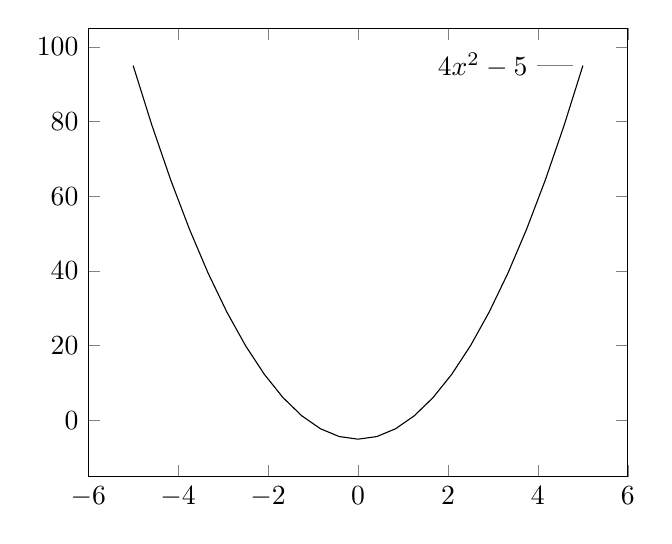
\begin{tikzpicture}
      \begin{axis}            % das Koordinatensystem wird mit
                              % der Umgebung axis erzeugt
          \addplot[             % ein Plot wird hinzugefügt
            domain=-5:5         % der Definitionsbereich
          ] { 4*x^2-5 }         % die Funktion
          node [pin=180:{$4x^2-5$}]{}; % Legende der Grafik
      \end{axis}
  \end{tikzpicture}
